%Chapter "Computational aspects"
%
\graphicspath{ {./img/Computational/} }
\chapter{FEM formulation of the elasticity BVP}
\label{chap: Computational Aspects}

\section*{Preliminary}
The previous chapter covered the boundary value problem for the model of theory of elasticity. It was shown that the model could equivalently be written in strong form (i.e., governing equations and boundary conditions) or in weak form. It was also shown that a particular interpretation of the weak form was that of the principle of virtual displacements. In this chapter we start from this principle and use interpolation theory to approximate both physical and virtual functions. As a result, this weak form of the BVP becomes a system of linear equations in the interpolation parameters that artificially enforce the principle of virtual displacements. The resulting finite element equations are shown to be equivalent to those governing the mechanical equilibrium of a discrete system of particles. To facilitate conceptual understanding we find first the equations for a single element and then proceed to consider the full mesh after invoking equilibrium and displacement compatibility conditions along element interfaces.

At the end of this chapter\footnote{{\bf This chapter, together with theoretical and computational learning activities is complemented by Jupyter Notebooks 8 through 12 available at the course REPO.}} the student should be able to:


\begin{itemize}
\item[•] Use interpolation theory to write the finite element based discrete version of the principle of virtual work.

\item[•] Recognize the finite element equilibrium equations of the elasticity BVP as physically analogous to those of a discrete system of particles.

\item[•] Understand the computational steps required for the implementation of the finite element. equilibrium equations in a computer language like Python.

\item[•] Understand the approximate nature of finite element solutions.

\end{itemize}

\section{FE algorithm starting from the weak formulation of the BVP}
In the previous chapter it was shown that the elasticity BVP could equivalently be formulated in differential and integral form in a so-called weak formulation. In this section we show that a simple finite element algorithm can be obtained if one introduces discretization, through the use of interpolation theory, into this weak form. Discretization appears in two forms: first, when one assumes that a primary variable is known at discrete (nodal) points and second when the interpolation functions exist over finite sub-domains or elements. For completeness we start by recalling the weak formulation introduced previously and then use our combined index notation for scalar components of tensorial functions and for componentes of nodal variables. The weak form is then given as follows:

Given the body forces $f_i$, the surface tractions $t_i^{\hat n}$ prescribed over the part of the boundary $S_t$ and the surface displacements ${\bar u_i}$ prescribed over the part of the boundary $S_u$ find the displacement field ${u_i}:V \to \mathbb{R}$ and such $\forall {w_i} \in V$ it satisfies:
\[\intL_V \sigma_{ij} w_{i,j}\, \dd{V} - \intL_V f_i w_i\, dV  - \intL_{S_t} t_i^{\hat n} w_i\, \dd{S} = 0.\]


In the expression above $V$ represents the complete problem domain while $S_t$ is that part of the boundary over which tractions are prescribed. Assume now that the full domain $V$ is divided into $NUMEL$ non-overlapping sub-domains (or finite elements) as shown schematically in \cref{fig:blow2}


\begin{figure}[h]
\centering
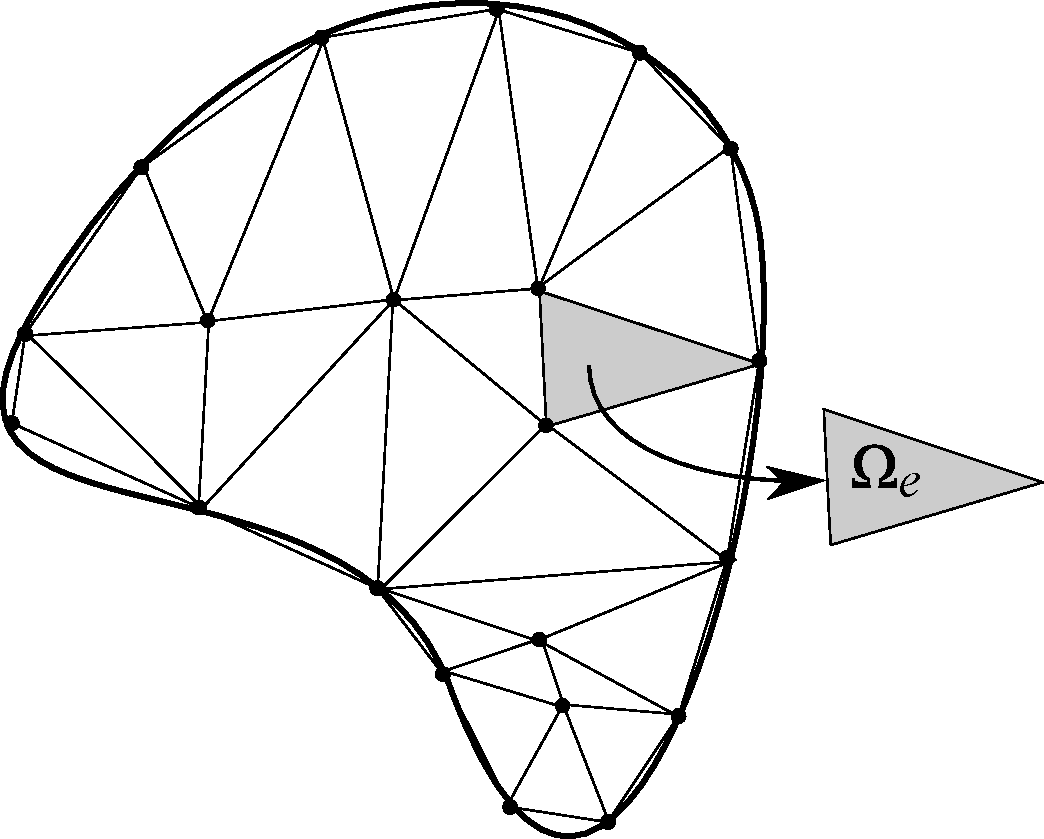
\includegraphics[width=8cm]{meshblow.pdf}
\caption{Meshed blow}
\label{fig:blow2}
\end{figure}


and in such a way that mathematically this can be expressed like:

\[V=\bigcup \Omega _e\]

and where $\Omega _e$ represents the sub-domain occupied by one such an element.

\begin{tcolorbox}
In the original strong form of the BVP the partial differential equations result from equilibrium arguments valid over infinitesimal material points occupying the domain $V$. In the FEM the operation of dividing the full domain $V$ into {\bf NUMEL} subdomains is equivalent to rendering the continuous problem with infinite material points into a discrete problem with a finite number of elements. In conclusion, a finite element is the discrete approximation of an infinitesimal material point.

\end{tcolorbox}


Note that each element is defined by an ordered set of nodal points establishing a prescribed interpolation space and used to conduct function approximations. In this element partition adjacent elements are connected through the nodal points in such a way that interpolation functions exist only within its element but are continuous through element interfaces. Using this partition in the weak form of equilibrium and using a summation symbol yields;

\[\sum_e\int_{\Omega_e}\sigma_{ij}w_{i,j}\operatorname d\Omega_e-\sum_e\int_{\Omega_e}f_iw_i\operatorname d\Omega_e-\sum_e\int_{S_e}t_iw_i\operatorname dS_e = 0\]


which is still the same form of the weak equilibrium expression.

In a second discretization operation we use interpolation methods to approximate both, the displacement field $u_i$ and the weighting function $w_i$ over each element as discussed previously. In particular assume that inside every element the fields can be approximated like:


\begin{align*} 
u_i(\overrightarrow x)& =N_i^Q(\overrightarrow x)\widehat u^Q \\ 
w_i(\overrightarrow x)& =N_i^Q(\overrightarrow x)\widehat w^Q
\end{align*}

and where $u^Q$ represent the scalar components of the displacement vector at the nodal point $Q$, $N_i^Q(\overrightarrow x)$ is the shape function for the nodal point $Q$ evaluated at the field point $\overrightarrow x$ and $u_i(\overrightarrow x)$ is the interpolated approximation to the displacement vector at the field point $\overrightarrow x$.


\begin{tcolorbox}
Recall that in expressions like

\[u_i(\overrightarrow x) =N_i^Q(\overrightarrow x)\widehat u^Q\]

the repeated super-script $Q$ implies summation over $Q= 1,..,Nnodes$ where $Nnodes$ is the number of nodes of the element.


\end{tcolorbox}

Considering the displacement field as the primary variable we can write in terms of the elastic constitutive tensor:

\[\sigma_{ij}=C_{ijkl}\varepsilon_{kl}\equiv C_{ijkl}B_{kl}^Q(\overrightarrow x)\widehat u^Q\]

after using

\begin{align*} 
\varepsilon_{ij}(\overrightarrow x)=B_{ij}^Q(\overrightarrow x)\widehat u^Q \\ 
w_{(i,j)}(\overrightarrow x)=B_{ij}^Q(\overrightarrow x)\widehat w^Q
\end{align*}


and where

\[ B_{ij}^Q(\overrightarrow x)=\frac12\left[\frac{\partial N_i^Q}{\partial x_j}+\frac{\partial N_j^Q}{\partial x_i}\right].\]

Substitution of the above in the discretized weak form gives us for an arbitrary $e$-element of domain $\Omega_e$

\[\widehat w^P\int_{\Omega_e}B_{ij}^PC_{ijkl}B_{kl}^Q\operatorname d\Omega_e\widehat u^Q-\widehat w^P\int_{\Omega_e}N_i^Pf_i\operatorname d\Omega_e-\widehat w^P\int_{S_e}N_i^Pt_i^{(n)}\operatorname ds_e=0.\]


Note that $w_i$ in the above expression is an arbitrary function and it is convenient to assign values like

\[\widehat w^T=\begin{bmatrix}0\cdots&1\cdots&0\end{bmatrix}\]

in turn  for every node in order to cancel the common term $\widehat w^P$ in such a way that we can write for an arbitrary $P$ degree of freedom:

\[\int_{\Omega_e}B_{ij}^PC_{ijkl}B_{kl}^Qd\Omega_e\widehat u^Q=\int_{\Omega_e}N_i^Pf_id\Omega_e+\int_{S_e}N_i^Pt_idS_e.\]

In this expression the dummy superscripts imply a summation over the number of nodes of the element in such a way that the only free index is $P$ which in this compact notation implies also that we have a system of equations corresponding to $P= 1,..,Nnodes$, which is the number of nodes of the element. Note also that the term $K_e^{PQ}$ defined by

\[K_e^{PQ}=\int_{\Omega_e}B_{ij}^PC_{ijkl}B_{kl}^Q\operatorname d\Omega_e\]


represents the force along degree of freedom $P$ due to a unit displacement along degree of freedom $Q$. In this sense we can define the following set of nodal forces along the $P$-th degree of freedom:

\begin{align*} 
f_\sigma^P & =K_e^{PQ}\widehat u^Q \\
f_B^P & =\int_{\Omega_e}N_i^Pf_i\operatorname d\Omega_e \\
f_c^P & =\int_{S_e}N_i^Pt_i^{(n)}\operatorname dS_e
\end{align*}

satisfying


\begin{equation}
f_\sigma^P=f_B^P+f_C^P
\label{nodal_forces}
\end{equation}


and where $f_\sigma^P$, $f_B^P$ and $f_C^P$ are forces due to the internal element stresses, body forces and surface tractions respectively.

\Cref{nodal_forces} which can also be written like:

\[K_e^{PQ}\widehat u^Q =f_B^P+f_C^P\]

is an equation in the nodal displacement $u^Q$ . However it must be observed that this equation has been derived for a single element $\Omega_e$ and the possible contribution in terms of forces and stiffness terms from additional elements is yet to be considered. This final step, leading to the assembly of the global system of equilibrium equations (to be discussed later) gives:


\begin{equation}
\left[K^G\right]\left\{U^G\right\}=\left\{RHS^G\right\}
\label{globalsys}
\end{equation}

and where the term $RHS^G$ is a vector of assembled global forces of the type $f_B^P+f_C^P$ storing the contribution from body forces and external surface tractions.

\begin{tcolorbox}
The details of the Python implementation of the stiffness matrix:

\[K_e^{PQ}=\int_{\Omega_e}B_{ij}^PC_{ijkl}B_{kl}^Q\operatorname d\Omega_e\]

are presented as an in-class activity in Notebook 6. This activity requires prior knowledge of interpolation (see Notebook 3) and numerical integration.

\end{tcolorbox}

\section{FE algorithm starting from the principle of virtual work}

As shown in the previous chapter a valid solution $(u_i , \sigma_{ij} , \epsilon_{ij})$ to the well-posed boundary value problem in theory of elasticity and where $u_i={\overline u}_i \quad \text{in} \quad  S_u$

satisfies 

\begin{equation}
\int\limits_V \sigma _{ij}\var{\varepsilon_{ij}}\dd{V}  - \int\limits_V f_i\delta u_i\dd{V}  - \int\limits_{S_t} t_i^{(n)}\var{u_i}\dd{S}  = 0
\label{PVDs}
\end{equation}

for arbitrary functions $\delta u_i$ such that  $\delta u_i =0 \quad \text{in} \quad  S_u$ and where:

\[\delta\varepsilon_{ij}=\frac12\left(\frac{\partial\delta u_i}{\partial x_j}+\frac{\partial\delta u_j}{\partial x_i}\right).\]

After using the same arguments and interpolation scheme as in the weak form discretization \cref{PVDs} leads to:


\[\int_{\Omega_e}B_{ij}^PC_{ijkl}B_{kl}^Qd\Omega_e\widehat u^Q=\int_{\Omega_e}N_i^Pf_id\Omega_e+\int_{S_e}N_i^Pt_idS_e\]

which is the same equation resulting from the discretization of the weak form.

Note that the PVW statement is an scalar (energy) equation relating the strain energy,

\[\delta E_s=\int_{\Omega_e}\sigma_{ij}\delta\varepsilon_{ij}\operatorname d\Omega_e\]

accumulated in the elastic solid as a result of the imposed virtual strain field $\delta\varepsilon_{ij}$ to the work of the external loads

\[\delta W=\int_{\Omega_e}f_i\delta u_i\operatorname d\Omega_e+\int_{S_e}t_i^{(n)}\delta u_i\operatorname dS_e\]

due to the imposition of the virtual displacement $\delta u_i$.

Using the same notation as in the previous algorithm the discrete version can also be written like:

\[\delta\widehat u^Pf_\sigma^P-\delta\widehat u^Pf_B^P-\delta\widehat u^Pf_c^P=0\]

and after using the arbitrariness in $\delta u_i$

\begin{equation}
f_\sigma^P-f_B^P-f_c^P=0.
\label{PVW_force}
\end{equation}


In a sense the FEM scheme makes use of interpolation theory to convert the continuous BVP governed by a set of partial differential equations into a discrete problem governed by a set of algebraic equations. Within this context \cref{PVW_force} can be interpreted as the force equilibrium equation governing the response of a particle $P$ subject to the action of:

\begin{itemize}
\item[•] External nodal forces $f_B^P$ consistent with body forces $f_i$.
\item[•] External nodal forces $f_c^P$ consistent with surface tractions $t_i^{(n)}$
\item[•] Internal forces $f_\sigma^P$ consistent with element stresses and equilibrating the external forces.
\end{itemize}

On the other hand, recall  that the PVW statement only holds if the set $(u_i , \sigma_{ij} , \epsilon_{ij})$ is the actual solution to the BVP. This fact implies that in the FE formulation where we only have an approximate solution $u_i(\overrightarrow x) =N_i^Q(\overrightarrow x)\widehat u^Q $ the principle does not hold as this is not the actual solution. However, the nodal displacements found after solving \cref{PVW_force} enforces such condition.

\begin{tcolorbox}

Since the finite element equation written in the form the term:

\[f_\sigma^P  =K_e^{PQ}\widehat u^Q\]

represents nodal forces equivalent to element stresses the coefficients $K_e^{PQ}$ represent the nodal force along degree of freedom $P$ due to a unit displacement along degree of freedom $Q.$

\end{tcolorbox}


\section{Global assembly}

The fundamental equation

\begin{equation}
K_e^{PQ}\widehat u^Q =f_B^P+f_c^P
\label{oneelement}
\end{equation}

resulting from the discretization of the PVW through the introduction of interpolation functions was derived over a single element of domain $\omega_e$. In order to consider the contribution from all the elements in a finite element discretized version of a solid we use Newton's third law of motion (action and reaction principle). For that purpose recall that the term $f_C^P$ in \cref{oneelement} corresponds to the contact forces resulting from surface tractions and it is computed according to:

\begin{equation}
f_c^P=\int_{S_t}N_i^Pt_i^n\operatorname dS
\label{traction}
\end{equation}

where it is evident that they depend on the external outward normal vector $\widehat n$ over $S_t$. Clearly, the mechanical interaction between two elements in contact takes place through these contact forces. To explain this interaction consider the schematic mesh shown in \cref{fig:4assembled1} below:


\begin{figure}[H]
\centering
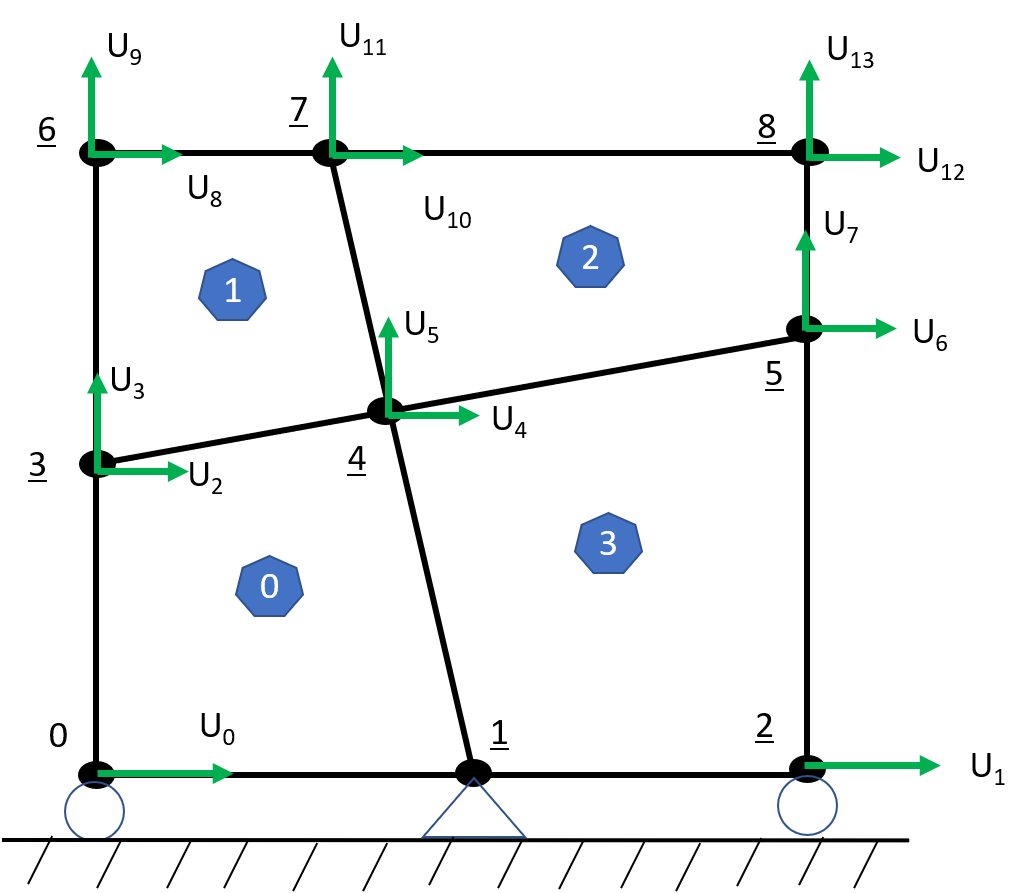
\includegraphics[width=8cm]{assembled}
\caption{4-elements mesh}
\label{fig:4assembled1}
\end{figure}


Focusing attention in elements $1$ and $2$ let the interacting surface be labelled as $S_b$ and extend this notation to the degrees of freedom and forces in such a way that the degrees of freedom of nodal points along $S_b$ would be named $U_b$ while those at other parts of the element would be named $U_c$. Accordingly the finite element equilibrium equations for each element can be written like:

\begin{equation}
\begin{Bmatrix}F_a\\F_b(\widehat n)\end{Bmatrix} = \begin{bmatrix}K_{aa}^1&K_{ab}^1\\K_{ba}^1&K_{bb}^1\end{bmatrix}\begin{Bmatrix}U_a\\U_b\end{Bmatrix}
\end{equation}

and

\begin{equation}
\begin{Bmatrix}-F_b(\widehat n\ast)\\F_C\end{Bmatrix}=\begin{bmatrix}K_{bb}^2&K_{bc}^2\\K_{cb}^2&K_{cc}^2\end{bmatrix}\begin{Bmatrix}U_b\\U_c\end{Bmatrix}
\end{equation}

The dependency of the contact forces along the common interface $S_b$ upon the normal outward vector $\widehat{n}$ has been made explicit in the equations. In particular this vector reads $\widehat n$ for element $1$ and ${\widehat n}^*$ for element $2$ and they satisfy:

\[\widehat n = - {\widehat n}^* . \]

Using this relation between the normal vectors at the contact interface we can write for the nodal forces:

\[ 
F_b(\widehat{n})+F_b({\widehat{n} }^*)=0
\]

or equivalently

\begin{equation}
F_b(\widehat n)-F_b(\widehat n)=0.
\label{coupling}
\end{equation}


This condition is shown for completeness in \cref{fig:coupled1}

\begin{figure}[H]
\centering
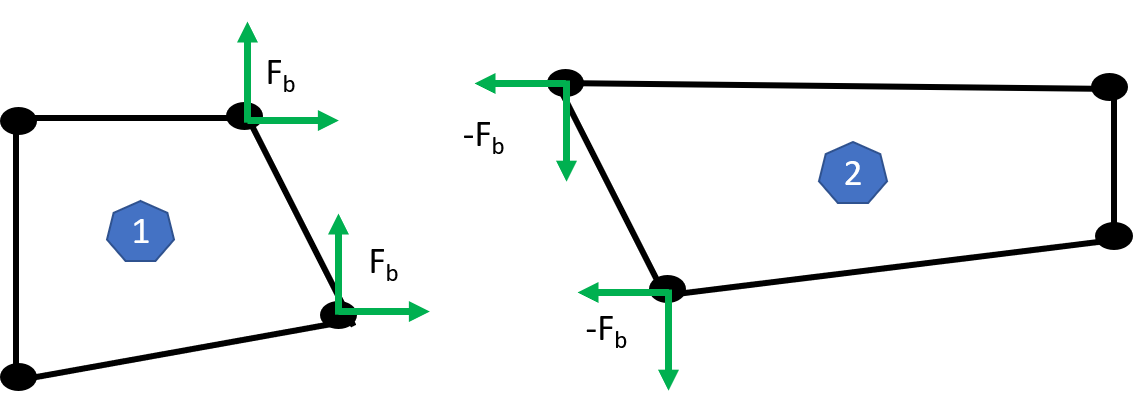
\includegraphics[width=12cm]{coupled1}
\caption{Equilibrated nodal forces along the contact interface $S_b$ of elements 1 and 2.}
\label{fig:coupled1}
\end{figure}

where it is evident that the contact nodal forces along element interfaces are equal and opposite in accordance with Newton's third law. On the other hand, from displacements continuity we have the condition:

\begin{equation}
U_B = U_B^1 = U_B^2.
\label{continuity}
\end{equation}

Using \cref{coupling} and \cref{continuity} in the equilibrium relationships yields the partial assemblage of the global stiffness matrix resulting after considering the interaction between elements $1$ and $2$:

\begin{equation}
\begin{bmatrix}K_{aa}^1&K_{ab}^1&0\\K_{ba}^1&K_{bb}^1+K_{bb}^2&K_{bc}^2\\0&K_{cb}^2&K_{cc}^2\end{bmatrix}\begin{Bmatrix}U_a\\U_b\\U_c\end{Bmatrix}=\begin{Bmatrix}F_a\\0\\F_c\end{Bmatrix}.
\label{finaleq}
\end{equation}

Note that in the right hand side vector from the above assembled global equilibrium equations only contact forces have been included. This process of adding elemental matrices through contact nodal forces is termed {\bf element assembly} and it is symbolically written like:

\begin{equation}\label{eq:assem}
{K^G}=\assem_{i=1}^{Numel} k^i
\end{equation}

and where $K^G$ is the global coefficient matrix; $k^i$ is the local elemental matrix for the $i$-th element; $\assem_{i=1}^{Numel}$ is the assembly operator and $i$ is an element index ranging between $1$ and the total number of elements $Numel$ that conform the finite element model. Notice that the assembly operator is analogous to a summation operator commonly used in the representation of series of finite or infinite number of terms, however in the finite element algorithm the assembly operator contains information indicating the position of each single term from the element coefficient matrix within the global system.

\begin{tcolorbox}

In most finite element codes the assembly operator is an array of integer values indicating the position (row and column) from each coefficient of the stiffness matrix of a given element. In {\bf SolidsPy} this operator is termed the {\bf DME()} operator and it is computed in the assembly module {\bf ASSEMUTIL}.

\end{tcolorbox}


\section{The assembly algorithm}

In this section we will discuss the fundamental algorithmic steps required for building the system of algebraic equations through the addition or assembly of elemental coefficient matrices as described by \cref{eq:assem}. This process of assembly of the elemental coefficient matrices into the global system involves:

\begin{itemize}
\item (i) The identification of the active degrees of freedom (or equation numbers) assigned to each node in the mesh.
\item (ii) The identification of the relationship between the elemental degrees of freedom and the global degrees of freedom.
\item (iii) The computation of the coefficient matrix for each element in the model.
\end{itemize}

\begin{tcolorbox}

In the finite element jargon the word {\bf elemental} commonly refers to variable or computations performed at the element level.

\end{tcolorbox}


Step (i) is easily accomplished by assigning a boundary condition flag to the degrees of freedom existing at each node indicating if the degree of freedom is active, in which case it contributes with an equation, or if it is prescribed, in which case it contributes with a specified displacement boundary condition. In our notation we use a $0$ value to indicate an active degree of freedom and a $-1$ value to indicate a prescribed degree of freedom. In the Python based code {\bf SolidsPy} this information is stored in a boundary conditions array termed $IBC$ and with dimensions $nn \times MDIM$, where $nn$ corresponds to the  total number of nodal points and $MDIM$ represents the problem dimensionality. The $IBC$ array is first given to the program through an input data file and later translated from $0$s and $-1$s to equation numbers. Thus during this process the boundary condition flag is read and equations are counted and numbers assigned according to the result. If the boundary condition flag is equal to $0$ the program assigns an equation number while it retains a $-1$ value for a $-1$ flag. In summary, the $IBC$ array exists in two instances. In its first instance it just contains integer flags indicating active or restrained degrees of freedom at each node while in a second instance it indicates the actual active equations existing at each node.

In parallel and also with data given through an input file, the nodes conforming each element are stored in a {\bf connectivity} array termed $IELCON$ and of dimension $Numel \times MxNNel$ where $Numel$ is the number of elements in the model and $MxNNel$ is the maximum number of nodes in a given element. Thus each row in the $IELCON$ array stores the nodal point data for the element. Each entry in the $IELCON$ array can now be directly translated into equation numbers using the processed version of the $IBC$ array. This process results in the discrete version of the assembly operator $\assem_{i=1}^{Numel}$ also called the assembly list or the $DME$ operator in {\bf SolidsPy}.

In the final step the mesh is looped one element at a time and each elemental coefficient matrix is assembled into the global matrix using the information (equation numbers) stored in the $DME$ operator. The actual computation of the elemental matrix is conducted by an element based subroutine, called $UEL$ in {\bf SolidsPy}. These subroutines may be different for each element in the mesh according to different kinematic o material assumptions. The assembly process is further illustrated by the following sample problem.

\paragraph*{Example}
For the mesh shown in \cref{fig:quad} where the elements are numbered from left to right and bottom to top write:

\begin{itemize}
\item (i) The boundary conditions array {\bf IBC()} in its two instances.
\item (ii) The connectivities array for the mesh.
\item (iii) The assembly {\bf DME()} operator.
\end{itemize}

\begin{figure}[h]
\centering
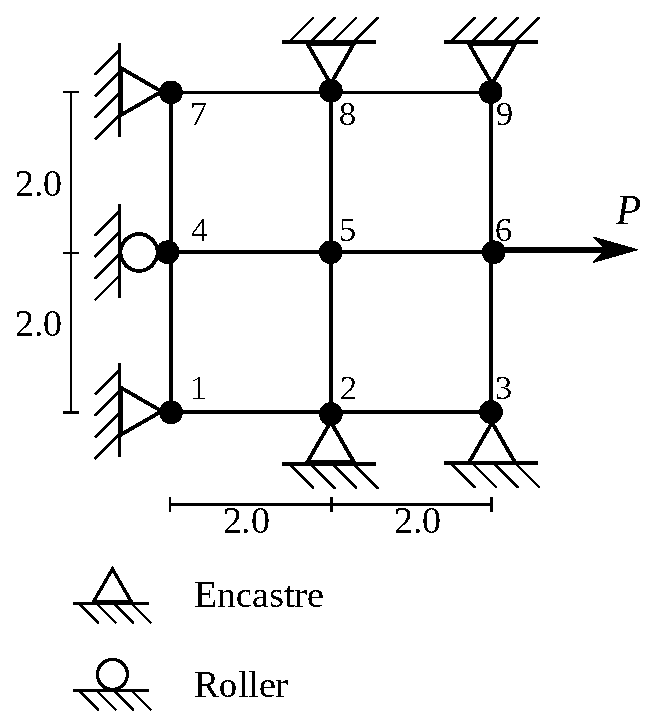
\includegraphics[width=8cm]{mesh2.pdf}
\caption{Mesh of 4 bi-linear finite elements.}
\label{fig:quad}
\end{figure}

(i) In a first instance the boundary conditions array {\bf IBC()} is filled with data assigned by the user in the input file. Since all the nodes in the bottom and top faces of the mesh are restrained in the horizontal and vertical directions they are assigned the flag $-1$ in each column. Similarly, node 4 is restrained only in the horizontal direction so it is assigned a $-1$ in the first position and a $0$ in the second position, while nodes 5 and 6 are completely free along both directions and they are assigned values of $0$. The resulting array is given by:

\[IBC_1 = \begin{bmatrix}
-1 & -1\\
-1 & -1\\
-1 & -1\\
-1 & 0\\
0 & 0\\
0 & 0\\
-1 & -1\\
-1 & -1\\
-1 & -1
\end{bmatrix}\]

In a second instance the boundary conditions array {\bf IBC()} is modified by the program which reads every value retaining those corresponding to $-1$ and assigning sequential numbers to those corresponding to $0$. Accordingly the first equation identified as $U_0$ corresponds to the vertical displacement of nodal point 4 while the remaining 4 equations associated to degrees of freedom $U_1 , U_2 , U_3 , U_4$ are the horizontal and vertical displacements of nodes 5 and 6. The final form of the array is given like: 

\[IBC_2 = \begin{bmatrix}
-1 & -1\\
-1 & -1\\
-1 & -1\\
-1 & 0\\
1 & 2\\
3 & 4\\
-1 & -1\\
-1 & -1\\
-1 & -1
\end{bmatrix}\]


(ii) The next step corresponds to the creation of the connectivities array {\bf IELCON()} storing the nodal points defining each element. In this case each element is defined by a list of 4 nodal point numbers. Recall that for the computation of the elemental stiffness matrix each element in the physical mesh is mapped to the canonical element in the natural space. In the natural space the shape functions are associated to a fixed node numbering and element orientation. If one follows a counter-clockwise orientation the node numbering must follow the same counter-clockwise orientation in the physical space. However the selection of the first node in the sequence is arbitrary and the mapping into the natural space will take care of the corresponding rotation. In this case a valid connectivities array is that given by:


\[IELCON = \begin{bmatrix}
0 &1 &4 &3\\
1 &2 &5 &4\\
3 &4 &7 &6\\
4 &5 &8 &7
\end{bmatrix}\]

(iii) The final ingredient required for the assembly of the global system of equations is the so-called {\bf DME()} operator. This is actually the same {\bf IELCON()} array but translated into equation numbers assigned at each element. Computationally this involves a subroutine that runs over the {\bf IELCON()} array, reads the value of the nodal identifier and then extracts the assigned equation numbers from the boundary conditions array {\bf IBC()}. In this example the assembly operator consistent with the definition of the connectivities array corresponds to:

\[DME = \begin{bmatrix}
-1 &-1 &-1 &-1 &1 &2 &-1 &0\\
-1 &-1 &-1&-1 &{\bf 3} &4 &1 &2\\
-1 &0 &1 &2 &-1 &-1 &-1 &-1\\
1 &2 &3 &4 &-1 &-1 &-1 &-1
\end{bmatrix}\]

\paragraph*{A note on the assembly operator:}
The definition of the element connectivities and its subsequent translation into degrees of freedom is carried out according to the local or canonical element definition in the natural space(\cref{fig:locdof})

\begin{figure}[H]
\centering
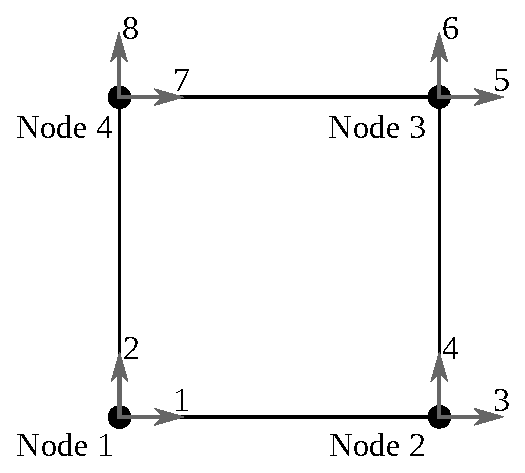
\includegraphics[width=6cm]{localdof.pdf}
\caption{Local definition for a 4-noded element.}
\label{fig:locdof}
\end{figure}

As a result the $(i,j)$ entry in the $DME$ array corresponds to the global equation number associated with the local degree of freedom $j$ of the $i$ element. For instance the value of $3$ stored at position $(1,4)$ in the current {\bf DME()} operator indicates that the global equation $3$ corresponds to the local equation $4$ (column index) in element $1$ (row index).

The assembly process is then conducted by identifying the relation between the entries in each row of the {\bf DME()} operator and the list of local degrees of freedom for the reference element shown in \cref{fig:locdof}. Accordingly, for element 1 it follows that the assembly of row $4$ of the local stiffness matrix proceeds as follows:
\begin{align*}
K_{3,3}^G & \leftarrow  K_{3,3}^G + k_{4,4}^1 \\
K_{3,4}^G & \leftarrow  K_{3,4}^G + k_{4,5}^1 \\
K_{3,1}^G & \leftarrow  K_{3,1}^G + k_{4,6}^1
\end{align*}


\section{Summary: The finite element algorithm}
At this point it becomes evident that the algorithm for the displacements based finite element method reduces to the solution of a linear system of algebraic equations in the unknown nodal displacements $U^G$ resulting after assembling the contribution to the stiffness matrix $K^G$ and loads vector $RHS^G$ from all the elements in the mesh. This process can be summarized in the 4-steps pseudo-code described in \cref{algo:overall1}:


\begin{algorithm}[H]
\SetAlgoLined
\KwData{Finite element model}
\KwResult{Field function}
\BlankLine
PREPROCESSING (Reads the model and computes {\bf IBC()}, {\bf IELCON()} and {\bf DME()} arrays);\\
ASSEMBLY (Forms the system of equations $\left[K^G\right]\left\{U^G\right\}=\left\{RHS^G\right\}$);\\
SOLUTION (Finds $U^G$);\\
POSTPROCESSING (Scatter the global solution to the elements and computes element forces, strains, and stresses);\\
\caption{Global steps involved in the finite element algorithm}
\label{algo:overall1}
\end{algorithm}

In the pre-processing stage the code reads the input file and forms the arrays {\bf IBC()}, {\bf IELCON()} and {\bf DME()} which are required for the assembly process. Once the global system of equations is assembled and solved, the values of the nodal displacements are distributed to the corresponding elements in a process commonly referred to like scattering. This process is somehow inverse to the assembly operation. With the nodal displacements for each element at hand it is now possible to compute nodal forces together with strain and stress distributions inside the element. The assembly and solution process is given in \cref{algo:overall2}. In this algorithm it must be noticed that the local stiffness matrix for each $i$ element is obtained by the call to the local element subroutine {\bf UEL()}.

\begin{algorithm}[H]
\SetAlgoLined
\KwData{Finite element model}
\KwResult{Field function}
\BlankLine
READ {\bf IBC()} and {\bf IELCON()} arrays from input files ;\\
COMPUTE modified {\bf IBC()} array ;\\
COMPUTE {\bf DME()} operator (using {\bf IBC()} and {\bf IELCON()} arrays);\\
INITIALIZE Global stiffness matrix $K^G \leftarrow 0.0$;\\
(Start assembly)
\BlankLine
\For{$i \leftarrow 1$ to $Numel$}{
    Call UEL(element parameters;$k^i$) ;\\
    $K^G \leftarrow K^G+^i$ (Assemble each $k^i$ into $K^G$ according to the {\bf DME()} operator);\\
    $RHS^G \leftarrow RHS^G+rhs^i$ (Assemble each $rhs^i$ into $RHS^G$);\\	
	\BlankLine
	}
\BlankLine
SOLVE ${K^G}{U^G} = RH{S^G}$;\\
Scatter nodal displacements solution to the elements
\caption{Details of the assembly and system solution process}
\label{algo:overall2}
\end{algorithm}

The details of the elemental subroutine {\bf UEL()} are given in \cref{algo:uel}. This process basically involves looping through the Gauss points and computing the required terms. The computation of the the strain-displacements matrix $B(r_j , s_j )$ and Jacobian determinant $\left\|J_j\right\|$ at each Gauss point is conducted by additional subroutines.

\newpage
\begin{algorithm}[H]
\SetAlgoLined
\KwData{Material parameters, nodal coordinates, applied loads}
\KwResult{$k^l$ and $rhs^l$}
\BlankLine
INITIALIZE $k^l \leftarrow 0.0$ ;\\
COMPUTE constitutive tensor $C_{ijkl}$ ;\\
FORM Gauss quadrature arrays $w()$ and $r() , s()$;\\
(Start loop through the Gauss points)
\BlankLine
\For{$j \leftarrow 1$ to $Ngpts$}{
    RETRIEVE $r_j$ , $s_j$ , $w_j$   ;\\ 
    COMPUTE $\left\|J_j\right\|$, $B(r_j , s_j )$ ;\\
    $k^l \leftarrow k^l+B^T C B \left\|J_j\right\| \left\|J_j\right\|$ ;\\
	\BlankLine
	}
\BlankLine
\caption{Details of the elemental {\bf UEL} subroutine}
\label{algo:uel}
\end{algorithm}


%\section{Sparse assembly}
%In Finite Elements is common to have stiffness and mass matrices that are sparse, i.e., matrices in which most of the elements are zero.
%
%
%For instance, in a regular mesh formed with bilinear quadrilaterals the number of nonzero entries is given by the expression
%\[\text{storage} = 9 n_x n_y - 9 n_x - 3 n_y + 4\, ,\]
%where $n_x$ is the number of nodes in the $x$ coordinate and $n_y$ is the number of nodes in the $y$ coordinate. Figure \ref{fig:sparse_storage} presents the needed storage for a mesh with $n_x=n_y$ for different sizes.
%\begin{figure}[H]
%\centering
%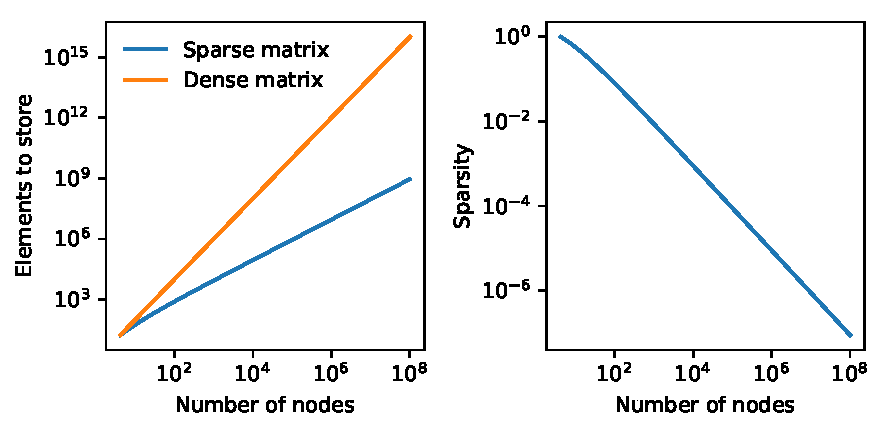
\includegraphics[width=6 in]{sparse_storage.pdf}
%\caption{Nonzero entries in a sparse matrix for a structured mesh of bilinear elements.}
%\label{fig:sparse_storage}
%\end{figure}



\paragraph*{Proposed problems}
\begin{enumerate}

\item \label{punto01} In the bi-linear element shown in \cref{fig:onemesh} the nodal displacements resulting from a finite element solution are indicated by the blue arrows. For the material parameters given in the figure find the nodal forces consistent with the element stresses. Assume plane strain behaviour.


\begin{figure}[H]
\centering
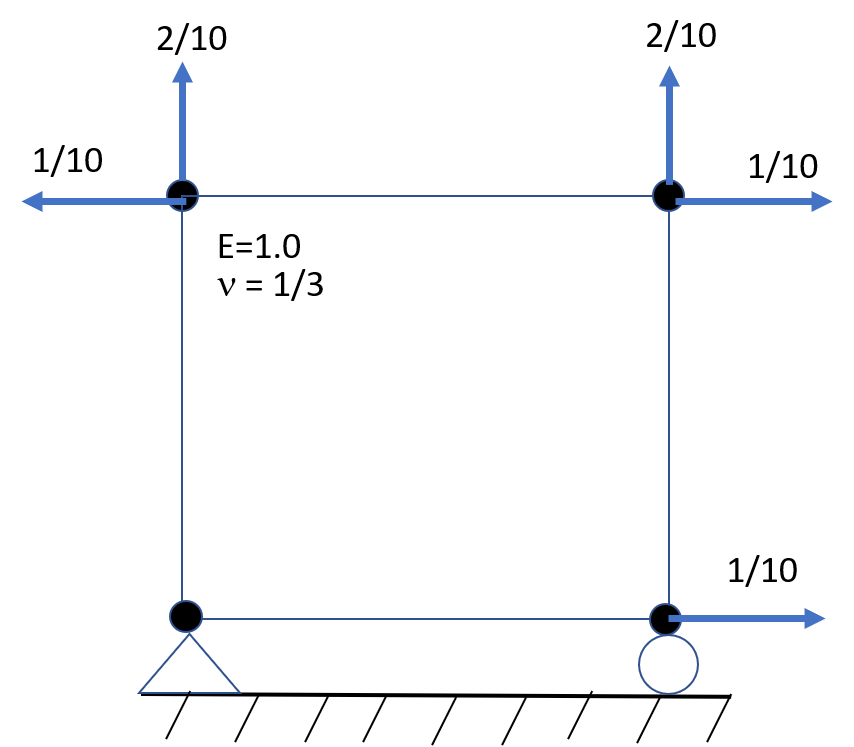
\includegraphics[height=6cm]{post.png} 
\caption{One-element mesh for problem 1.}
\label{fig:onemesh}
\end{figure}


\item \label{punto02} For the mesh shown in the figure, with internal surfaces between elements 1-3 and 3-2 labelled $S_b$ and $S_c$ respectively, write the form of the global stiffness matrix resulting from the physical assembly. Explicitly formulate the force and displacement compatibility equations along both boundaries


\begin{figure}[H]
\centering
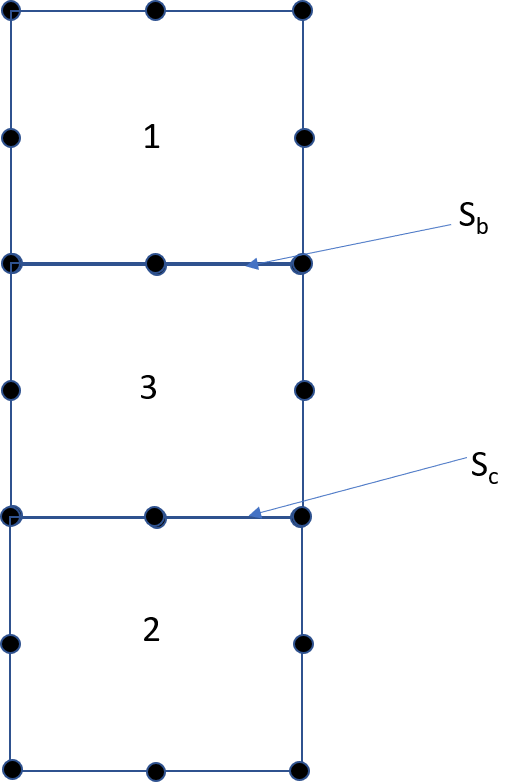
\includegraphics[height=6cm]{long.png} 
\caption{Long mesh for problem 2.}
\label{fig:longmesh}
\end{figure}

\item \label{punto03} For the mesh shown in the figure propose different node numbering schemes and identify the resulting changes in the size of the half-band in the stiffness matrix. Assume that each element subroutine is full of $1$s.

\begin{figure}[H]
\centering
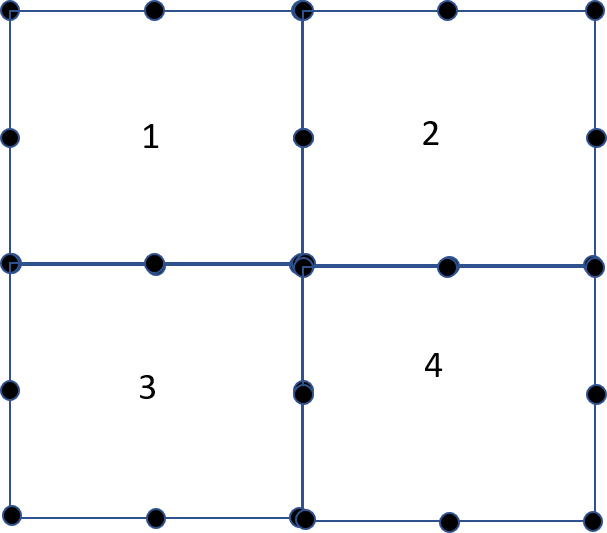
\includegraphics[height=6cm]{halfband.png} 
\caption{Long mesh for problem 3.}
\label{fig:halfmesh}
\end{figure}



\item \label{punto04} A finite element model is conformed by an assemblage of three elements of the type shown in \cref{fig:cercha}


\begin{figure}[H]
\centering
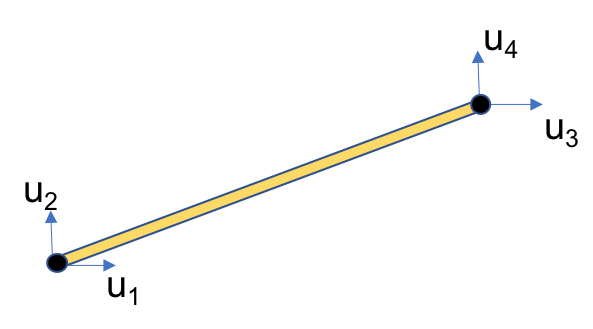
\includegraphics[height=3cm]{truss.png} 
\caption{Fundamental element}
\label{fig:cercha}
\end{figure}

and with a stiffness matrix (in the global coordinate system) given by:

\[
k = \begin{bmatrix}1&1&1&1\\1&1&1&1\\1&1&1&1\\1&1&1&1.
\end{bmatrix}
\]

On the other hand, it is known that global stiffness matrix has been assemble using the following operator

\[
DME = \begin{bmatrix}-1&-1&2&3\\-1&-1&1&-1\\1&-1&2&3\end{bmatrix}
\]

in which a value of $-1$ refers to a restrained degree of freedom and thus equal to zero. It is required to:

\begin{itemize}
\item Draw the complete model including its displacement boundary conditions.
\item Indicate the order of the global stiffness matrix for the complete structure.
\item Find the global stiffness matrix for the structure.
\end{itemize}





%%%%%
\item \label{punto05} Using SolidsPy compute the stress concentration factor defined according to:

\[SCF = \frac{\max\, \sigma_{yy}}{\text{promedio}\, \sigma_{yy}}\, \]

and introduced after drilling a hole in the following plates:

\begin{figure}[H]
	\centering
	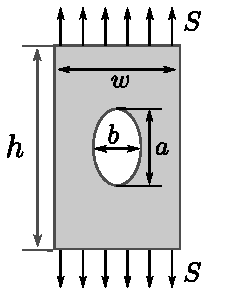
\includegraphics[height=5 cm]{tema1.pdf}
	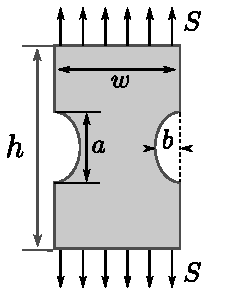
\includegraphics[height=5 cm]{tema2.pdf}
	\caption{Plates with holes.}
	\label{fig:tema1}
\end{figure}

In both cases the material parameters are defined in \cref{tab:comun}

\begin{table}[H]
    \centering
    \begin{tabular}{cc}
        \hline
        Parameter & Value \\
        \hline
        Young's modulus (Pa)    & $E =200 \times 10^9$ \\
        Poisson's ratio    & $\nu = 0.285$   \\
        Load (N/m)   & $S = 10^8$  \\
        \hline
    \end{tabular}
    \caption{Material parameters for the analysis defined in problem 2.}
    \label{tab:comun}
\end{table}

while the geometric parameters are those of \cref{tab:tema1}

\begin{table}[H]
	\centering
	\begin{tabular}{cccc}
		\hline
		$a$ & $b$ & $h$ & $w$ \\
		\hline
		20      & 40      & 50      & 100  \\
		\hline
	\end{tabular}
	\caption{Geometric parameters for the analysis defined in problem 2.}
	\label{tab:tema1}
\end{table}




%\inputminted[]{python}{src/engine.py}




%En este caso el factor de concentración de esfuerzos ($SCF$) se calcula como:
%
%
%\subsection*{Tema 2}
%\begin{figure}[H]
%	\centering
%	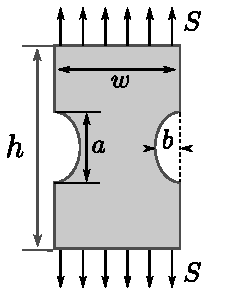
\includegraphics[height=5 cm]{tema2.pdf}
%	\caption{Geometrías y condiciones del tema 2.}
%	\label{fig:tema2}
%\end{figure}
%\begin{table}[H]
%	\centering
%	\begin{tabular}{ccccc}
%		\hline
%		Equipo & $a$ & $b$ & $h$ & $w$ \\
%		\hline
%        3    & 40      & 40      & 50      & 100  \\
%        10   & 20      & 40      & 50      & 200  \\
%        14   & 10      & 20      & 50      & 100  \\
%        16   & 20      & 40      & 50      & 100  \\
%        21   & 10      & 40      & 100     & 200  \\
%        24   & 10      & 40      & 100     & 300  \\
%        28   & 10      & 30      & 100     & 200  \\
%		\hline
%	\end{tabular}
%	\caption{Equipos y parámetros para el tema 2. Longitudes en milímetros. Considere las simetrías del problema para que esté cinemáticamente determinado.}
%	\label{tab:tema2}
%\end{table}
%
%En este caso el factor de concentración de esfuerzos ($SCF$) se calcula como:
%\[SCF = \frac{\max\, \sigma_{yy}}{\text{promedio}\, \sigma_{yy}}\, .\]
%
%\subsection*{Tema 3}
%\begin{figure}[H]
%	\centering
%	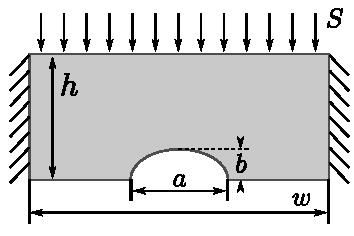
\includegraphics[height=4 cm]{tema3.pdf}
%	\caption{Geometrías y condiciones del tema 3.}
%	\label{fig:tema3}
%\end{figure}
%\begin{table}[H]
%	\centering
%	\begin{tabular}{ccccc}
%		\hline
%		Equipo & $a$ & $b$ & $h$ & $w$ \\
%		\hline
%		2   & 20      & 10      & 50      & 200  \\
%		6   & 10      & 10      & 50      & 200  \\
%		8   & 20      & 20      & 50      & 200  \\
%		13  & 10      & 20      & 50      & 200  \\
%		19  & 20      & 30      & 60      & 240  \\
%		25  & 20      & 40      & 60      & 240  \\
%		27  & 40      & 20      & 60      & 240  \\
%		\hline
%	\end{tabular}
%	\caption{Equipos y parámetros para el tema 3. Longitudes en milímetros.}
%	\label{tab:tema3}
%\end{table}
%
%En este caso el factor de concentración de esfuerzos ($SCF$) se calcula como:
%\[SCF = \frac{\max|\sigma_{xx}|}{\text{promedio}\, |\sigma_{xx}|}\, .\]
%
%\subsection*{Tema 4}
%\begin{figure}[H]
%	\centering
%	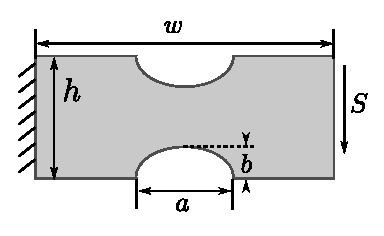
\includegraphics[height=4 cm]{tema4.pdf}
%	\caption{Geometrías y condiciones del tema 4.}
%	\label{fig:tema4}
%\end{figure}
%\begin{table}[H]
%	\centering
%	\begin{tabular}{ccccc}
%		\hline
%		Equipo & $a$ & $b$ & $h$ & $w$ \\
%        \hline
%        1   & 20      & 10      & 50      & 100  \\
%		7   & 20      & 10      & 50      & 200  \\
%		9   & 20      & 10      & 50      & 300  \\
%		15  & 10      & 10      & 50      & 100  \\
%		18  & 10      & 10      & 50      & 200  \\
%		20  & 10      & 10      & 50      & 300  \\
%		26  & 20      & 20      & 60      & 200  \\
%		\hline
%	\end{tabular}
%	\caption{Equipos y parámetros para el tema 4. Longitudes en milímetros.}
%	\label{tab:tema4}
%\end{table}
%
%En este caso el factor de concentración de esfuerzos ($SCF$) se calcula como:
%\[SCF = \frac{\max|\sigma_{xx}|}{\text{promedio}\, |\sigma_{xx}|}\, .\]



%%%%%



\end{enumerate}















